\section{Ray Tracing and Landau Damping}
\label{section:raytracing}
\subsection{Ray Tracing}
Whistler-mode waves in the magnetosphere propagate for very large distances, and with relatively little attenuation. Under certain conditions, these waves can persist from a few seconds to 1 or more minutes. Simulating the propagation of these waves using a full-wave method would be extremely intractable with current computational resources. However we can use ray tracing to approximate their behavior.

Ray tracing is a technique from geometric optics which tracks the position and velocity of a coherent wave packet -- essentially, approximate the behavior of a wave packet to that of a photon, and evaluate the packet's velocity and wavenormal vector with respect to time. Ray tracing is best suited for coherent, monochromatic wave packets, with no attenuation, dispersion, or mode coupling. 

Ray tracing was first applied to the Whistler mode by \cite{Haselgrove1955} using a graphical technique, then subsequently by \cite{Haselgrove1960} and \cite{Kimura1966} for numerical computation. These papers worked in curvilinear coordinates with respect to a magnetic field line. Haselgrove's Equations have been used extensively by numerous magnetospheric scientists \citep{Kimura1966, Edgar1972, Ngo1989,Ristic1993, Lauben1998, B.Peter2007, Bortnik2005, Kulkarni2009}, several using the so-called ``Stanford Ray Tracing Program'' -- a legacy Fortran code which evaluated the Haselgrove equations in two dimensions. Our work uses a slightly different code originally developed by Dr. Forrest Foust \citep{Golden2010}, and is designed for flexibility with respect to plasma density and magnetic field models. Rather than work in curvilinear coordinates with explicit derivatives, we adopt a more-general formulation, using a three-dimensional Cartesian frame and numerically-evaluated derivatives.

We begin with the fundamental ray-tracing equations, as given by \cite{Haselgrove1960, Stix1992}:

\begin{eqnarray}
\frac{d\vec{r}}{dt} = \frac{\nabla_kF}{\partial F/\partial \omega} \label{eqn:raytracing_position}\\
\frac{d\vec{k}}{dt} = \frac{\nabla_rF}{\partial F/\partial \omega} \label{eqn:raytracing_wavenormal} \\
\end{eqnarray}
Constrained such that:
\begin{equation}
F = F(\vec{r},t,\vec{k},\omega) = 0
\end{equation}
Equation \ref{eqn:raytracing_position} is simply $\frac{\nabla_kF}{\partial F/\partial \omega} \approx\frac{\partial F/\partial k}{\partial F /\partial \omega} = \frac{\partial \omega}{\partial k} = v_g$, the group velocity of a wave packet. The corresponding equation describing the evolution of the wavenormal vector (\ref{eqn:raytracing_wavenormal}) is less intuitive, although an analogy can be drawn to Hamiltonian mechanics, in which $\omega$ represents a velocity, and $k$ a momentum.

The function F, our ``conserved quantity'', is simply the cold plasma dispersion relation given by equation \ref{eqn:disp_rln}.

The raytracing equations are a set of coupled, first-order differential equations; solutions to which require some subtlety, but can be addressed using standard numerical techniques.

First, note that we can solve the set at a given time, then evolve the system forward some finite time step. However, the constraint $F=0$ may not be strictly held afterward. We assert that the error in this constraint must be small; which in turn implies that the background medium must be smoothly-varying -- i.e., changing on a spatial scale much greater than our forward step, and of the wavelength of interest. This assumption is known as the \emph{WKB Approximation}.
\begin{figure}[ht]
\begin{center}
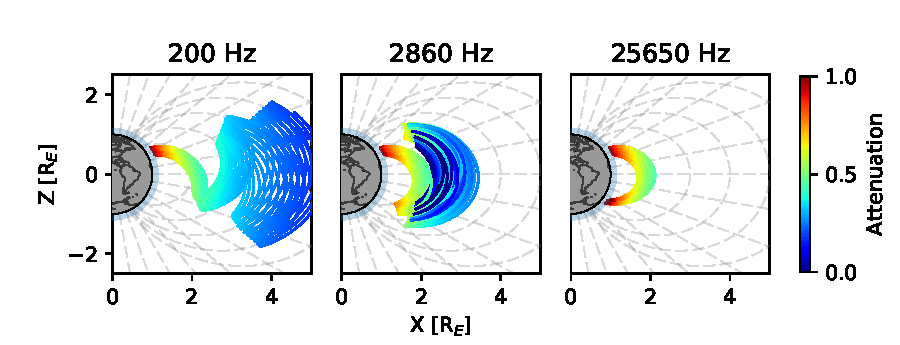
\includegraphics{Figures/raytracing_example.pdf}
\end{center}
\caption[Example ray tracing]{Example ray families as computed by the raytracer}
\end{figure}
\subsubsection{Adaptive Timestepping}
The process of raytracing, then, is to 1) solve the dispersion relation (\ref{eqn:disp_rln}) to find the refractive index; 2) compute the velocity vector and step the system forward in time; and 3) re-evaluate at the new position to assure that the condition F=0 remains held. However, properly selecting the timestep is of critical importance -- too large a timestep and positional errors will accumulate, or the ray will slip out of a propagating mode; too small and computational speed and memory usage suffers. We use an adaptive \emph{Runge-Kutta-Fehlberg} (RK45) \citep{Fehlberg1969, Mathews2004} method to continuously update the timestep as the raytracer progresses. RK45 is a common technique for solving ordinary differential equations.

The RK45 method approximates a solution with an initial stepsize $dt$ using two spline fits: a fourth-order and a fifth-order. The error in the step is taken to be the difference between the two estimates. If the error is above a specified tolerance $\epsilon$, the stepsize is reduced and the evaluation is repeated. Additionally, if the error is below a specified tolerance ($\epsilon/10$ in our implementation), the stepsize is increased. The result is a variable time axis with finer resolution in regions of high variability, while enabling longer timesteps in smooth regions for computational efficiency. See appendix \ref{appendix:runge_kutta} for a detailed description of the Runge-Kutta method.

\subsection{Landau Damping}
The cold-plasma formulation of raytracing described above evaluates the trajectory and wavenormal angle of a wave packet -- however, it assumes zero attenuation of wave energy. While it is possible to account for wave attenuation in ray tracing using warm plasma corrections \citep{Sazhin1993, Henyey1980}, we follow the same approximation as used in the legacy ray tracing code, and calculate attenuation along the cold-plasma raypath according to Landau damping.

Landau damping, originating in a seminal work by \cite{Landau1946}, is a resonant interaction between a wave and the distribution of electrons and ions comprising the background medium. The Landau mechanism is an interaction with parallel streaming particles and the wave's electric field. Resonant particles are accelerated or decelerated by the wave's electric field; if a majority of the resonant electrons have velocities slightly below that of the wave, then a coherent effect exists, the wavefront imparts some net energy to the plasma, and the wave is attenuated. Conversely, if the majority of resonant particles are moving faster than the wave, some of their energy can be imparted to the wavefront, inducing \emph{wave growth} \citep{Chen1983, Kulkarni2009}. 

Landau damping can have multiple resonances (in which the particle has multiple complete rotations per rotation of the wave). The lowest resonant mode is known as the \emph{Landau} resonance, while the $\pm 1$ modes are referred to as the \emph{Cyclotron} resonances. Higher-order modes remain nameless.

We use the expressions for Landau damping as formulated by \cite{Brinca1972}. \citeauthor{Brinca1972} derived expressions for Landau damping assuming a cold background plasma with a sparse warm distribution added, for Whistler waves propagating at an arbitrary angle to the background magnetic field. Inputs to this formulation are the familiar Stix parameters (equations \ref{eqn:stix_params_1} - \ref{eqn:stix_params_2}), which are in turn a function only of location and wave frequency; the wavenormal angle with respect to the background magnetic field; and a distribution function which specifies the energies (and thus velocities) of thermal electrons. The full set of Landau damping equations is given in appendix \ref{appendix:landau}.

Interestingly, \citeauthor{Brinca1972}'s work was motivated by measurements of Whistler-mode wave growth, rather than attenuation. Our implementation follows suit, and is equally capable of returning growth or damping, depending on the plasma model used. However, throughout this research, wave growth has been exceedingly rare.

\subsubsection{Thermal electron distributions}

The extent to which a wave is amplified or damped is heavily dependent on the energy distribution of background electrons. The energy distribution, or temperature profile, is specified as a normalized function in phase space -- a function of position and velocity, which is normalized to 1:

\begin{eqnarray}
f  & = & f(\vec{r}, \vec{v}, t) \\
& =  & f(\vec{r}, v_\perp, v_\parallel, t) \\
\int_0^\infty f d v_\perp & = & 1 \\
\end{eqnarray}

Two distribution functions are used in similar work -- the \cite{Bell2002} distribution, which was derived from POLAR spacecraft measurements of the inner plasmasphere, and the \cite{Bortnik2007} distribution, which is based on CRRES spacecraft measurements above L $\approx$ 7.

We use the phase space density function as described in \cite{Golden2010}, which smoothly transitions between the \cite{Bell2002} model inside the plasmapause, and the \cite{Bortnik2007} model outside the plasmapause. Figure \ref{fig:phase_space_density} shows an example of the distribution function.

\begin{figure}[ht]
\begin{center}
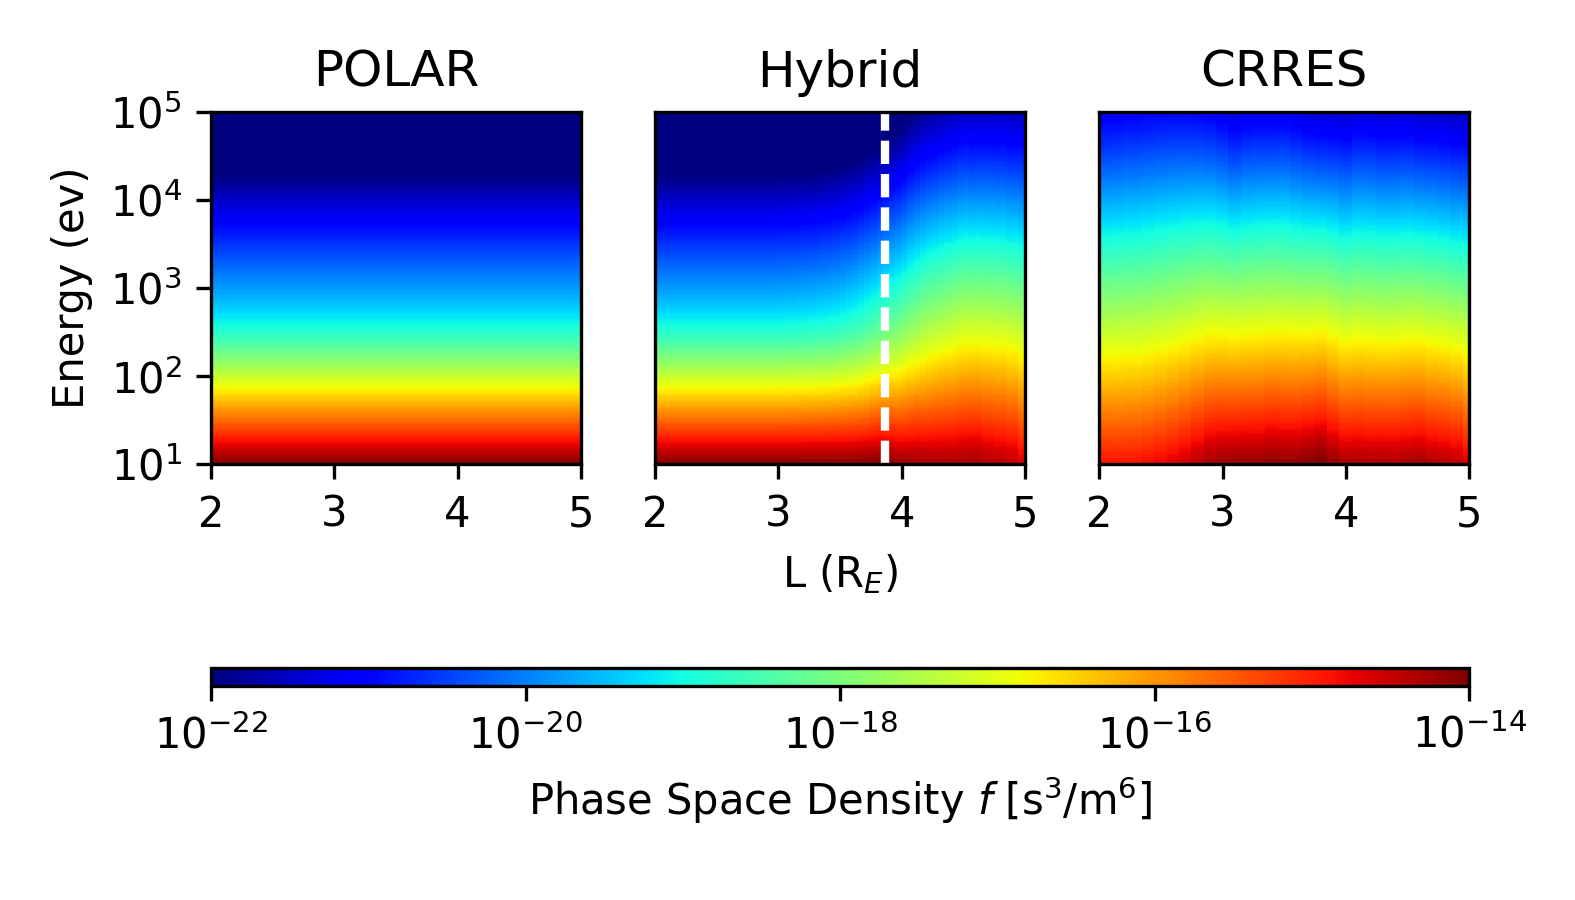
\includegraphics{Figures/psd.png}
\end{center}
\caption[Phase-space density functions]{Example phase-space density functions, shown for $A_e$=1.6, $K_p$=4, $\alpha$=45$^\circ$, and MLT=18. The POLAR model is used inside the plasmapause, and the CRRES model outside the plasmapause. The hybrid model smoothly transitions between the two. The plasmapause, at $L\approx 4$, is marked by the dashed white line.}
\label{fig:phase_space_density}
\end{figure}







